\documentclass{article}

% Workshop submission: switch to [dblblindworkshop] (or [sglblindworkshop])
% and set \workshoptitle{...} when a target workshop is fixed. We use the
% [preprint] option here to keep the draft venue-neutral.
\usepackage[preprint, nonatbib]{neurips_2026}

\usepackage[utf8]{inputenc}
\usepackage[T1]{fontenc}
\usepackage{hyperref}
\usepackage{url}
\usepackage{booktabs}
\usepackage{amsmath}
\usepackage{amsfonts}
\usepackage{amssymb}
\usepackage{microtype}
\usepackage{xcolor}
\usepackage{graphicx}
\usepackage{tikz}
\usetikzlibrary{positioning, arrows.meta, calc}

% Compact display math
\setlength{\abovedisplayskip}{4pt}
\setlength{\belowdisplayskip}{4pt}
\setlength{\abovedisplayshortskip}{2pt}
\setlength{\belowdisplayshortskip}{2pt}

\title{Metal-Sci: A Scientific Compute Benchmark for\\Evolutionary LLM Kernel Search on Apple Silicon}

\author{%
  Anonymous Authors \\
  Anonymous Affiliation \\
  \texttt{anonymous@example.org}
}

\begin{document}
\maketitle

\begin{abstract}
LLM-driven code search has produced impressive results on GPU ML kernels (GEMM,
attention, convolution), but the optimization patterns in scientific computing
are systematically different: bandwidth-bound stencils with halo tiling,
register-blocked all-pairs interactions, multi-field Boltzmann updates,
neighbour-list molecular dynamics with atomics, parallel-chain MCMC,
multi-kernel nonlinear PDE solvers, and butterfly/data-shuffle spectral
transforms. We present \textsc{Metal-Sci}, a 10-task benchmark of
scientific Apple-Silicon Metal compute kernels spanning six optimization
regimes. Every task ships a CPU reference, a roofline ceiling,
and a naive but correct seed; the fitness signal is the geometric mean of
\emph{achieved/ceiling} across three problem sizes, with any tolerance
failure forcing the score to zero. We release the harness and seeds and report a uniform
10-iteration Claude Opus~4.7 sweep over all ten tasks on Apple M1~Pro.
In-distribution speedups span $1.00\times$ to $10.6\times$.
\emph{The held-out evaluation is sharper than the in-distribution
one and exposes overfitting that the geometric mean hides.} On HMC,
the \texttt{template <uint D>} dispatch that took $d{=}8$ from 121 to
970\,GFLOPS hard-codes branches for $d{\in}\{8,16,32\}$ and
\emph{returns wrong answers} at the held-out $d{=}24$. On LBM, a
$32{\times}2$ threadgroup geometry tuned for the training sizes
regresses to $0.64\times$ of the seed at $192^2$. gradshaf, lj,
fft3d, and nbody extrapolate cleanly. Metal-specific syntax
(\texttt{[[max\_total\_threads\_per\_threadgroup]]} attribute
placement, \texttt{half} as reserved fp16 keyword, MSL's lack of
C++ lambdas) recurs as an out-of-distribution failure across
iterations. The benchmark is designed for fast iteration: each
candidate compiles, runs, verifies, and scores in seconds.
\end{abstract}

\section{Introduction}

LLM code-search systems --- FunSearch~[1], AlphaEvolve~[2], and recent
kernel-generation work~[3] --- evaluate language models as
\emph{optimisers} of executable artefacts. The choice of artefact matters:
KernelBench targets PyTorch ML kernels (GEMM, attention, convolution) on
CUDA, where canonical implementations are heavily represented in
pretraining data and the optimisation surface is dominated by tiling and
warp-level reductions.

Scientific computing exposes a different surface. Stencils are
bandwidth-bound and reward halo and temporal blocking. All-pairs
interactions are compute-bound and reward register blocking with
shared-memory cooperative loads. Lattice Boltzmann ping-pongs nine
distribution functions per cell with non-trivial pull-stream indexing.
Cell-list molecular dynamics touches irregular memory through atomic
counters. Hamiltonian Monte Carlo runs many chains in parallel where
register pressure scales with the problem dimension $d$. Grad-Shafranov
solvers chain a max-reduction with a variable-coefficient stencil. 3D
FFTs are dominated by data-shuffle/butterfly patterns and twiddle-factor
caching rather than tiling. Each pattern stresses a distinct dimension of
the compiler/memory hierarchy, and canonical optimisations~[5,6,7,8,11]
differ regime-to-regime.

We target Apple Silicon's Metal compute pipeline. It is underrepresented
in CUDA-centric training data --- frontier models reliably mishandle
Metal-specific syntax such as the
\texttt{[[max\_total\_threads\_per\_threadgroup]]} kernel attribute, a real
out-of-distribution generalisation test. Its unified memory model removes
host-device copy plumbing, enabling sub-second compile-run-verify cycles
per candidate that are essential for fast evolutionary loops. And it
supports rich simdgroup intrinsics (\texttt{simd\_max},
\texttt{simd\_broadcast}) and threadgroup-memory tiling, giving the LLM a
non-trivial optimisation surface.

\paragraph{Contributions.} (i) A 10-task scientific compute benchmark over
six optimisation regimes, each with a CPU reference, roofline-anchored
fitness, and multi-size generalisation gate. (ii) A runtime-compiled
harness that exposes compile errors, correctness diagnostics, and per-size
GPU timing back to the LLM. (iii) Preliminary evolution runs across Claude
Opus~4.7 and Gemini~3 on M1 Pro, qualitatively analysing which patterns
each model recovers.

\section{Benchmark tasks}
\label{sec:tasks}

Each task ships (a) a Metal source describing the problem, (b) a naive
correct seed, (c) a CPU reference with task-specific tolerance, (d) three
in-distribution sizes plus one held-out size, and (e) a roofline ceiling
in either GFLOPS (compute-bound) or GB/s (bandwidth-bound). Tasks are
grouped by optimisation regime.

\subsection{Regular stencils (regime R1)}

\paragraph{heat2d.} Two-dimensional heat equation, 5-point stencil on
$(N_x{\times}N_y)$ grid with Dirichlet boundaries. Per timestep, per
interior cell:
\begin{equation}
u^{n+1}_{i,j} \;=\; u^n_{i,j} + \alpha\!\left(u^n_{i-1,j}+u^n_{i+1,j}
   + u^n_{i,j-1}+u^n_{i,j+1} - 4\,u^n_{i,j}\right).
\end{equation}
Bandwidth-bound at 8\,B/cell; tests halo handling and temporal blocking.

\paragraph{wave3d.} Three-dimensional acoustic wave equation, 7-point
isotropic Laplacian, leapfrog in time:
\begin{equation}
u^{n+1}_{i,j,k} = 2u^n_{i,j,k} - u^{n-1}_{i,j,k}
   + \alpha\,\big(u^n_{i\pm 1,j,k}+u^n_{i,j\pm 1,k}+u^n_{i,j,k\pm 1}-6\,u^n_{i,j,k}\big),
\end{equation}
where each $\pm$ expands to two terms. CFL stability requires
$\alpha=(c\Delta t/\Delta x)^2<1/3$ (we use $0.18$). 12\,B/cell unique
DRAM traffic. Tests register pressure, 2.5D blocking, and marching-axis choice.

\subsection{Compute-bound (regime R2)}

\paragraph{nbody.} All-pairs gravitational $N$-body with leapfrog. Per
body $i$ per step:
\begin{equation}
\mathbf{a}_i \;=\; G\sum_{j} m_j
   \frac{\mathbf{r}_j-\mathbf{r}_i}
        {(\|\mathbf{r}_j-\mathbf{r}_i\|^2+\varepsilon^2)^{3/2}},
\quad \mathbf{v}\!\mathrel{+}\!=\mathbf{a}\Delta t,
\quad \mathbf{r}\!\mathrel{+}\!=\mathbf{v}\Delta t.
\end{equation}
Self-interaction is masked by the softening $\varepsilon$. $\sim$20\,FLOPs
per pair; ceiling at peak FP32 GFLOPS. Tests register blocking and
threadgroup cooperative loads.

\paragraph{hmc.} Hamiltonian Monte Carlo on an anisotropic Gaussian target,
$U(q)=\tfrac12 q^\top A q$ with $A=\Sigma^{-1}$. One thread per chain;
many chains in parallel. Each HMC step draws $p\sim\mathcal{N}(0,I)$ and
runs $L$ leapfrog inner steps with stepsize $\varepsilon$,
\begin{equation}
p \leftarrow p - \tfrac{\varepsilon}{2}A q,\quad
q \leftarrow q + \varepsilon p,\quad
p \leftarrow p - \varepsilon Aq,\ \cdots,\quad
p \leftarrow p - \tfrac{\varepsilon}{2}A q,
\end{equation}
followed by a Metropolis accept/reject with $\log u_{\mathrm{acc}}<-\Delta H$.
Correctness is verified statistically (sample mean and Frobenius covariance
error vs.\ the target). Three sizes $(d,K)\in\{(8,16{\rm K}),(16,4{\rm K}),(32,1{\rm K})\}$
probe the register-pressure boundary; at $d{=}32$ per-thread state
($\sim$512\,B) competes with the register file.

\subsection{Multi-field, exotic memory (regime R3)}

\paragraph{lbm.} D2Q9 Lattice Boltzmann, fused pull-stream + BGK
collision, periodic BC. With velocity table $\mathbf{c}_k$ and weights
$w_k$, per cell per step:
\begin{align}
f^{\mathrm{str}}_k(\mathbf{x})
   &= f^{\mathrm{in}}_k(\mathbf{x}-\mathbf{c}_k),\quad
\rho = \textstyle\sum_k f^{\mathrm{str}}_k,\quad
\mathbf{u} = \tfrac{1}{\rho}\sum_k \mathbf{c}_k\,f^{\mathrm{str}}_k, \\
f^{\mathrm{eq}}_k &= w_k\rho\!\left(1+3(\mathbf{c}_k{\cdot}\mathbf{u})
   +\tfrac{9}{2}(\mathbf{c}_k{\cdot}\mathbf{u})^2 - \tfrac{3}{2}\|\mathbf{u}\|^2\right),\\
f^{\mathrm{out}}_k &= f^{\mathrm{str}}_k - \tau^{-1}\!\left(f^{\mathrm{str}}_k - f^{\mathrm{eq}}_k\right).
\end{align}
Storage is SoA: $f[k\,N_xN_y + jN_x + i]$. $72$\,B/cell DRAM traffic.
Tests AoS/SoA layout, push vs pull streaming, and algebraic
factorisations of the BGK kernel.

\paragraph{ising.} Two-dimensional Ising model, checkerboard Metropolis
Monte Carlo on a periodic $N_x\times N_y$ lattice with $\sigma\in\{\pm 1\}$
stored as int8. Per attempt at site $(i,j)$:
\begin{equation}
h = \sigma_{i\pm 1,j}+\sigma_{i,j\pm 1}\in\{-4,\ldots,4\},\quad
\Delta E = 2J\sigma\,h,\quad
\mathrm{accept}\iff u<\exp(-\beta\,\Delta E).
\end{equation}
A precomputed five-entry $p_{\mathrm{accept}}$ table and a counter-based
Murmur-fmix32 PRNG yield bit-exact CPU/GPU agreement: verification is
byte-equality on the spin array. $2$\,B/site/sweep ceiling.

\subsection{Irregular memory and atomics (regime R4)}

\paragraph{lj.} Lennard-Jones molecular dynamics with a cell-list spatial
hash. Three kernels per step --- \texttt{clear\_cells}, \texttt{build\_cells}
(atomic scatter), \texttt{step} (27-neighbour-cell pair force + integration):
\begin{equation}
\mathbf{F}_i = \sum_{j\in\mathcal{N}(i)} -24\!\left(2r_{ij}^{-12}-r_{ij}^{-6}\right)r_{ij}^{-2}\,(\mathbf{r}_j-\mathbf{r}_i),
\qquad r_{ij}<r_{\mathrm{cut}}=2.5,
\end{equation}
with minimum-image periodic wrap. Cell occupancy is built via
\texttt{atomic\_fetch\_add} on a per-cell counter. Tests load balancing,
atomic contention, and the irregular access patterns of neighbour-list MD.

\subsection{Multi-kernel reductions (regime R5)}

\paragraph{gradshaf.} Grad-Shafranov fixed-boundary equilibrium via Picard
iteration, two kernels per outer step: an interior max-reduction
$\psi_{\mathrm{axis}}=\max_{(i,j)\in\mathrm{int}}\psi$, then a
variable-coefficient 5-point stencil with nonlinear source:
\begin{align}
\psi_{\mathrm{norm}} &= \psi/\psi_{\mathrm{axis}},\quad
J = R\,p_{\mathrm{axis}}\cdot 4\psi_{\mathrm{norm}}(1-\psi_{\mathrm{norm}})\cdot
   \mathbf{1}[0<\psi_{\mathrm{norm}}<1],\\
\Delta^*\psi &= a_W\psi_W+a_E\psi_E+a_N\psi_N+a_S\psi_S+a_C\psi_C,\\
\psi^{n+1} &= \psi^n + \omega\,(-\mu_0 R J - \Delta^*\psi)/a_C,
\end{align}
with $R$-dependent $a_{W,E}=1/dR^2 \pm 1/(2RdR)$, $a_{N,S}=1/dZ^2$,
$a_C=-2(1/dR^2+1/dZ^2)$. Tests in-kernel reduction strategies (single-TG
vs simdgroup-tree) and multi-kernel composition.

\subsection{Data-shuffle / butterfly (regime R6)}

\paragraph{fft3d.} 3D complex-to-complex forward FFT, fp32, on a
power-of-two cube of side $N$. Convention is unnormalised (matches
\texttt{numpy.fft.fftn}); storage is row-major \texttt{float2}$[N][N][N]$.
Three named kernels --- \texttt{fft3d\_x}, \texttt{fft3d\_y},
\texttt{fft3d\_z} --- are dispatched in sequence with two ping-ponged
buffers, each kernel performing a length-$N$ 1D FFT per threadgroup of
$N$ cooperating threads:
\begin{equation}
Y[k_1,k_2,k_3] \;=\; \sum_{n_1,n_2,n_3=0}^{N-1} X[n_1,n_2,n_3]\,
   \exp\!\left(-\frac{2\pi i}{N}(k_1 n_1 + k_2 n_2 + k_3 n_3)\right).
\end{equation}
Sizes $N \in \{32, 64, 128\}$ cover three working-set regimes: $32^3$
(${\sim}256$\,KB) is SLC-resident and compute-bound; $128^3$
(${\sim}16$\,MB) DRAM-binds. The optimisation surface is dominated by
data movement, not arithmetic --- bit-reversal vs Stockham auto-sort,
twiddle-factor caching, mixed-radix (radix-4, radix-8) butterflies for
fewer barriers, and \texttt{simd\_shuffle} / \texttt{simd\_shuffle\_xor}
for intra-simdgroup butterflies are all on the table. Tests
threadgroup-memory bank-conflict avoidance and the per-axis stride
asymmetry (stride 1 along $x$ vs strides $N$ and $N^2$ along $y$, $z$).
$\sim 5N\log_2 N$ FLOPs per 1D FFT; effective DRAM traffic 96\,B/cell
across the three axis passes (16\,B read + 16\,B write per pass).
Verification is max-norm against \texttt{numpy.fft.fftn} on a fixed
seeded Gaussian input, tolerance $10^{-3}{+}10^{-3}\|Y\|_\infty$.

A bandwidth-bound smoke-test (\texttt{saxpy}) is also included to validate
the harness.

\section{Harness}
\label{sec:harness}

\paragraph{Compile and dispatch.} The harness uses PyObjC's Metal bindings
and runtime-compiles \texttt{.metal} source via
\texttt{MTLDevice.newLibraryWithSource}, avoiding the offline
\texttt{xcrun metal} toolchain; compile errors are returned as structured
strings to the LLM. Buffers are allocated in unified memory; numpy views
alias buffer contents with a single copy on read-back. All dispatches for a
multi-size run share one \texttt{MTLCommandBuffer}, and timings come from
\texttt{GPUEndTime}\,$-$\,\texttt{GPUStartTime} (3 warmup, 10 timed,
median reported). The chip is detected from \texttt{sysctl} and looked up
in a per-family table (M1 through M4) for peak FP32 GFLOPS and DRAM
bandwidth; all runs here are on Apple M1 Pro (4500\,GFLOPS, 200\,GB/s).

\paragraph{Scoring.} For a candidate passing correctness at every size,
$S = \left(\prod_{i} f_i\right)^{1/n}$ with $f_i=\mathrm{achieved}_i/\mathrm{ceiling}_i$.
Any tolerance failure forces $S{=}0$; this hard gate prevents trading
correctness for speed, and the geometric mean across sizes discourages
overfitting to one regime.

\paragraph{Evolution loop.} A single-population $(\mu{=}1{+}\lambda{=}1)$
loop. Iteration $i$ shows the LLM the previous candidate, the incumbent
best, a short history per iteration, and the original task spec. The LLM
returns a Metal source block (multi-kernel tasks emit multiple
\texttt{kernel} functions in one file). Candidates strictly beating the
incumbent are promoted; prompts, raw responses, extended-thinking tokens,
sources, and per-size JSON results are persisted. A single
\texttt{call\_llm} bridge dispatches Claude via the Agent SDK and Gemini
via \texttt{google-genai}.

\section{Preliminary results}
\label{sec:results}

We run a uniform single-model sweep on Apple M1~Pro: claude-opus-4-7 over
each of the ten tasks for ten iterations, $\mu{=}1{+}\lambda{=}1$, no human
prompt intervention. Table~\ref{tab:results} reports the in-distribution
score (gmean $\mathrm{achieved}/\mathrm{ceiling}$ over the three training
sizes) and a held-out evaluation, in which the unmodified seed and the
incumbent best are run on a single unseen problem size declared by the
task spec (Sec.~\ref{sec:tasks}).

\begin{table}[t]
\caption{Uniform 10-iteration claude-opus-4-7 sweep, Apple M1~Pro.
``In-distribution'' = gmean(achieved/ceiling) over three training sizes;
correctness is a hard gate. ``Held-out'' = fraction-of-ceiling at the
unseen size, then ratio. lbm and wave3d use longer pre-existing runs
(25 and 15 iters).}
\label{tab:results}
\centering
\footnotesize
\setlength{\tabcolsep}{4pt}
\begin{tabular}{l rrr rrr l}
\toprule
       & \multicolumn{3}{c}{In-distribution} & \multicolumn{3}{c}{Held-out} & \\
\cmidrule(lr){2-4}\cmidrule(lr){5-7}
Task     & Seed & Best  & $\times$ & Seed & Best & $\times$ & Outcome \\
\midrule
saxpy    & 0.817 & 1.022 & 1.25  & 79\%   & 78\%   & 0.99           & saturated \\
heat2d   & 0.609 & 0.609 & 1.00  & 100\%  & 101\%  & 1.01           & saturated; no candidate beat seed \\
wave3d   & 0.533 & 0.673 & 1.26  & 97\%   & 94\%   & 0.97           & saturated \\
ising    & 0.066 & 0.075 & 1.13  & 12\%   & 11\%   & 0.96           & flat \\
fft3d    & 0.162 & 0.167 & 1.03  & 39\%   & 42\%   & 1.08           & generalises \\
nbody    & 0.019 & 0.055 & 2.83  & 1.0\%  & 1.7\%  & 1.63           & generalises \\
gradshaf & 0.022 & 0.041 & 1.89  & 3.1\%  & 5.8\%  & 1.89           & generalises (identical) \\
lj       & 0.003 & 0.005 & 1.77  & 0.25\% & 0.45\% & 1.77           & generalises (identical) \\
lbm      & 0.395 & 0.576 & 1.46  & 83\%   & 53\%   & \textbf{0.64}  & \textbf{regresses} (TG geom.) \\
hmc      & 0.009 & 0.093 & 10.6  & 0.55\% & ---    & \textbf{FAIL}  & \textbf{wrong answer} at $d{=}24$ \\
\bottomrule
\end{tabular}
\end{table}

\paragraph{In-distribution.} Speedups span $1.00\times$ to $10.6\times$.
The HMC step (Fig.~\ref{fig:hmc-evol}) is the high end: introducing a
\texttt{template <uint D>} worker dispatched on runtime $d$ at
iteration~6 moves $d{=}8$ from 121 to 970\,GFLOPS by enabling full
unroll of the inner $A\,q$ matvec. Saturated tasks (saxpy, heat2d,
wave3d) sit above 78\% of effective DRAM ceiling on the seed; heat2d
is the cleanest demonstration that the score is a \emph{hard} signal
--- zero candidates strictly dominated the seed across all three
sizes, so the incumbent stayed at iter~0.

\paragraph{Held-out generalisation is sharper than in-distribution.}
Three populations separate cleanly. (i)~\emph{Generalises}: nbody,
fft3d, gradshaf, lj. Gradshaf and lj held-out speedups match their
in-distribution speedups to two significant figures (size-invariant
simdgroup-tree reduction and cell-list traversal); fft3d $256^3$
extrapolates past the largest training size $128^3$.
(ii)~\emph{Saturated}: saxpy, heat2d, wave3d, ising --- nothing to win.
(iii)~\emph{Overfits}, in two qualitatively different ways.
\textbf{LBM} regresses to $0.64\times$ of the seed on the held-out
$192^2$ grid: the iter-23 best pins
\texttt{[[max\_total\_threads\_per\_threadgroup(64)]]} with a
$32{\times}2$ geometry tuned for the $\{64, 128, 256\}^2$ training
sizes; on a non-multiple of 32 the geometry wastes threads at the
boundary, and the BGK algebraic fold cannot recover the loss.
\textbf{HMC} \emph{fails correctness} at $d{=}24$: the template
specialisation dispatches \texttt{if (d==8) run<8>() ... else
run<32>()}, so $d{=}24$ lands in the $D{=}32$ branch; per-thread
\texttt{q[32], p[32]} and the unrolled matvec process 32 entries
against 24-entry data, and sample covariance lands ${\sim}10\sigma$
off target. The seed (runtime-$d$ loop) is correct on $d{=}24$ at
0.55\% of FP32 peak --- a specialisation/generalisation tradeoff the
held-out gate exposes and the in-distribution score hides. The LBM
$256^2$ result above 100\% of nominal ceiling reflects working-set
residency in the system-level cache: the 8\,B/cell roofline is
DRAM-only.

\paragraph{Recurring Metal-grammar failures.}
\texttt{[[max\_total\_threads\_per\_threadgroup(N)]]} is mis-placed
(after the parameter list, or as a standalone statement, instead of on
the \texttt{kernel void} declaration) on \emph{seven} candidates
across five tasks (saxpy, heat2d, nbody, ising, wave3d) ---
reproduced from earlier opus-4-6 and gemini-3.1-pro runs.
\texttt{half} is reserved as MSL's fp16 type, breaking
\texttt{uint half = N >> 1u;} on fft3d iters~1 and 6. C++ lambdas
are unsupported, tripping ising iter~2 and wave3d iter~15. Wave3d
shows the highest correctness failure rate (10/15): multi-step
leapfrog amplifies any sign or indexing error into NaN.

\begin{figure}[t]
\centering
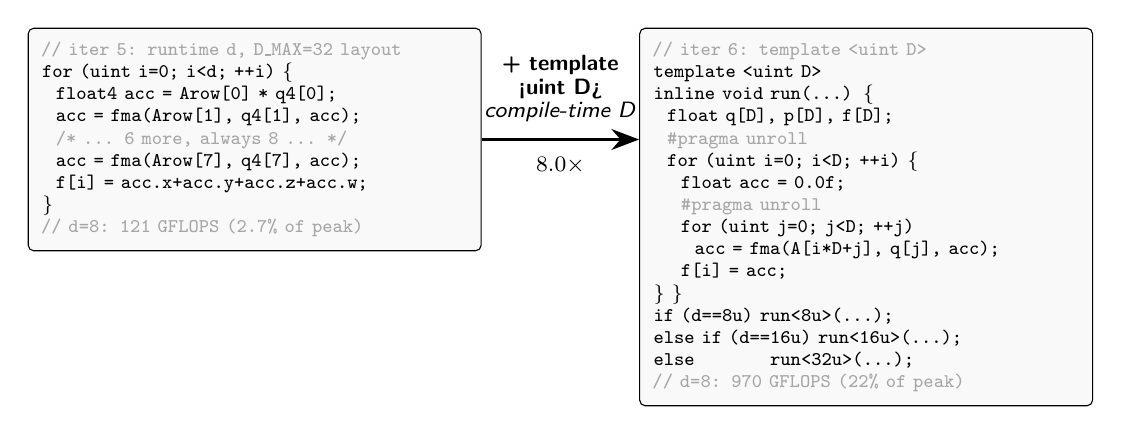
\begin{tikzpicture}[
  code/.style={draw, rounded corners=2pt, fill=gray!5,
               inner sep=5pt, align=left, font=\scriptsize\ttfamily,
               text width=54mm, anchor=north west},
  arr/.style={-{Stealth[length=3.5mm]}, line width=1.4pt},
]
\node[code] (l) at (0,0) {%
\textcolor{gray!70}{// iter 5: runtime d, D\_MAX=32 layout}\\
for (uint i=0; i<d; ++i) \{\\
\ \ float4 acc = Arow[0] * q4[0];\\
\ \ acc = fma(Arow[1], q4[1], acc);\\
\ \ \textcolor{gray!70}{/* ... 6 more, always 8 ... */}\\
\ \ acc = fma(Arow[7], q4[7], acc);\\
\ \ f[i] = acc.x+acc.y+acc.z+acc.w;\\
\}\\
\textcolor{gray!70}{// d=8: 121 GFLOPS (2.7\% of peak)}};

\node[code] (r) at ($(l.north east)+(20mm,0)$) {%
\textcolor{gray!70}{// iter 6: template <uint D>}\\
template <uint D>\\
inline void run(...) \{\\
\ \ float q[D], p[D], f[D];\\
\ \ \textcolor{gray!70}{\#pragma unroll}\\
\ \ for (uint i=0; i<D; ++i) \{\\
\ \ \ \ float acc = 0.0f;\\
\ \ \ \ \textcolor{gray!70}{\#pragma unroll}\\
\ \ \ \ for (uint j=0; j<D; ++j)\\
\ \ \ \ \ \ acc = fma(A[i*D+j], q[j], acc);\\
\ \ \ \ f[i] = acc;\\
\} \}\\
if (d==8u) run<8u>(...);\\
else if (d==16u) run<16u>(...);\\
else \ \ \ \ \ \ \ \ \ \ run<32u>(...);\\
\textcolor{gray!70}{// d=8: 970 GFLOPS (22\% of peak)}};

\coordinate (lm) at ($(l.east|-l.center)$);
\coordinate (rm) at (lm-|r.west);
\node[font=\footnotesize\sffamily, align=center, above=1mm of $(lm)!0.5!(rm)$]
  (lab) {\textbf{+ template}\\[-1pt]\textbf{<uint D>}\\[-1pt]\textit{compile-time D}};
\node[font=\footnotesize\sffamily\bfseries, below=1mm of $(lm)!0.5!(rm)$] {$8.0\times$};
\draw[arr] (lm) -- (rm);
\end{tikzpicture}
\caption{Paradigmatic candidate evolution: HMC, Opus~4.7, iter~5\,$\rightarrow$\,6.
The structural change is one declaration --- \texttt{template <uint D>}
with three runtime-dispatched instantiations $d\in\{8,16,32\}$. Iter~5 had a
manually-unrolled float4 inner loop against a fixed $D_{\max}{=}32$ layout
(over-computing at $d{=}8$, plus a 4-way horizontal sum); iter~6 sizes
\texttt{q,p,f} exactly to $D$ so both loops fully unroll into scalar FMAs ---
moving $d{=}8$ from 121 to 970\,GFLOPS in one iteration after five had
stalled at 2--4\% of peak.}
\label{fig:hmc-evol}
\end{figure}


\section{Discussion}

A roofline-anchored score answers ``how close are we to the hardware?'' in
physical units; the geometric mean across sizes is hard to game by
overfitting one regime. Apple Silicon's unified memory halves the host-side
scaffolding compared to CUDA, enabling sub-second compile-run-verify
cycles per candidate --- which matters more than it sounds: an evolutionary
loop with tens of candidates needs a fast \emph{harness}, not a fast kernel.
Metal's smaller, quirkier surface (simdgroup intrinsics, threadgroup
attributes) also surfaces OOD failures of CUDA-trained LLMs on tasks that
are otherwise textbook.

\paragraph{Limitations and future work.} The static per-chip ceilings do not
account for SLC residency at small sizes (see the LBM 256$^2$ result above);
a workload-aware roofline~[4] per task and per size would tighten the score.
The single-population $(1{+}1)$ loop plateaus within 10--25 iterations on
most tasks --- an island-model or FunSearch-style~[1] archive with a novelty
signal~[2] is the natural next step, particularly for the irregular-memory
tasks. Future tasks include sparse linear algebra (SpMV, CG) and
cross-chip generalisation (evolve on M2~Pro, evaluate on M3~Max).

\section*{References}
\footnotesize
\begin{itemize}\setlength{\itemsep}{0pt}\setlength{\parskip}{0pt}\setlength{\topsep}{0pt}
\item[\textnormal{[1]}] Romera-Paredes, B.\ et al.\ (2024) Mathematical
discoveries from program search with large language models. \emph{Nature}
\textbf{625}, 468--475.
\item[\textnormal{[2]}] Novikov, A.\ et al.\ (2025) AlphaEvolve: A coding agent
for scientific and algorithmic discovery. \emph{arXiv:2506.13131}.
\item[\textnormal{[3]}] Ouyang, A.\ et al.\ (2025) KernelBench: Can LLMs Write
Efficient GPU Kernels? \emph{arXiv:2502.10517}.
\item[\textnormal{[4]}] Williams, S., Waterman, A.\ \& Patterson, D.\ (2009)
Roofline: An insightful visual performance model for multicore architectures.
\emph{CACM} \textbf{52}(4), 65--76.
\item[\textnormal{[5]}] Datta, K.\ et al.\ (2008) Stencil computation
optimization and auto-tuning on state-of-the-art multicore architectures.
\emph{Proc.\ SC '08}.
\item[\textnormal{[6]}] Nyland, L., Harris, M.\ \& Prins, J.\ (2007) Fast
N-body simulation with CUDA. \emph{GPU Gems 3}, ch.\ 31.
\item[\textnormal{[7]}] Sch\"onherr, M.\ et al.\ (2011) Multi-thread
implementations of the lattice Boltzmann method on non-uniform grids for
CPUs and GPUs. \emph{Comput.\ Math.\ Appl.}\ \textbf{61}(12), 3730--3743.
\item[\textnormal{[8]}] Anderson, J.\ A., Lorenz, C.\ D.\ \& Travesset, A.\
(2008) General purpose molecular dynamics simulations fully implemented on
graphics processing units. \emph{J.\ Comput.\ Phys.}\ \textbf{227}(10),
5342--5359.
\item[\textnormal{[9]}] Micikevicius, P.\ (2009) 3D finite difference
computation on GPUs using CUDA. \emph{Proc.\ GPGPU-2}.
\item[\textnormal{[10]}] Geb, L.\ et al.\ (2022) Seamless GPU acceleration
for C++ based physics on the Apple M1's unified processing units.
\emph{arXiv:2206.01791}.
\item[\textnormal{[11]}] Govindaraju, N.\ K.\ et al.\ (2008) High
performance discrete Fourier transforms on graphics processors.
\emph{Proc.\ SC '08}.
\item[\textnormal{[12]}] Li, J.\ et al.\ (2025) TritonBench: Benchmarking
large language model capabilities for generating Triton operators.
\emph{Findings of ACL 2025}, pp.\ 23053--23066.
\item[\textnormal{[13]}] Saroufim, M.\ et al.\ (2025) BackendBench:
benchmarking PyTorch-backend kernel generation.
\item[\textnormal{[14]}] Wen, J.\ et al.\ (2025) MultiKernelBench:
multi-platform LLM kernel generation across CUDA, Ascend\,C, and Pallas.
\item[\textnormal{[15]}] Kalade, S.\ \& Schelle, G.\ (2025) NPUEval:
optimising NPU kernels with LLMs and open-source compilers.
\emph{arXiv:2507.14403}.
\item[\textnormal{[16]}] Nie, J.\ et al.\ (2026) KernelCraft: benchmarking
agentic close-to-metal kernel generation on emerging hardware.
\emph{arXiv:2603.08721}.
\item[\textnormal{[17]}] Lange, R.\ T.\ et al.\ (2025) Towards robust
agentic CUDA kernel benchmarking, verification, and optimisation.
\emph{arXiv:2509.14279}.
\item[\textnormal{[18]}] Guo, P.\ et al.\ (2025) EvoEngineer: mastering
automated CUDA kernel evolution with large language models.
\emph{arXiv:2510.03760}.
\end{itemize}

\appendix

\section{Related work}
\label{app:related}

\subsection{LLM-driven kernel-generation benchmarks}

A wave of benchmarks has emerged for evaluating LLMs as generators of
high-performance GPU kernels. \emph{KernelBench}~[3] targets PyTorch ML
kernels (GEMM, attention, convolution, normalisation, activation) on
CUDA and scores single-shot generation by speedup against the PyTorch
eager baseline. \emph{TritonBench}~[12] extends to the Triton DSL and
adds reference code-similarity to correctness and performance.
\emph{BackendBench}~[13] evaluates correctness alone for kernels written
against the PyTorch backend interface. \emph{MultiKernelBench}~[14]
broadens the platform set to CUDA, Ascend\,C, and Pallas while retaining
the ML-operator workload set. \emph{NPUEval}~[15] targets the AMD AIE
NPU in C++ and exposes a tool-use feedback loop with multi-turn
regeneration. Most recently, \emph{KernelCraft}~[16] benchmarks
bare-metal assembly kernel generation on emerging accelerator ISAs
(PLENA, AMD NPU, Coral NPU, Sonic BOOM), with native tool interfaces
(\texttt{check\_syntax}, \texttt{run\_evaluation}, \texttt{view\_output},
\texttt{grep\_docs}) and a three-tier ML-task taxonomy (primitive,
composite, end-to-end). Across these benchmarks the workload is ML and
the headline number is speedup against a vendor or compiler baseline.

\subsection{LLM-driven evolutionary code search}

The broader paradigm of LLMs as \emph{optimisers} inside evolutionary
code-search loops was established by \emph{FunSearch}~[1] for
symbolic-algorithm discovery and scaled by \emph{AlphaEvolve}~[2] across
mathematical and algorithmic domains. \emph{AI CUDA Engineer}~[17] and
\emph{EvoEngineer}~[18] specialise this paradigm to CUDA kernel
optimisation, replacing single-shot or agentic regeneration with a
population/archive driven by a fitness signal --- closer in spirit to
our $(\mu{=}1{+}\lambda{=}1)$ loop, but on CUDA ML kernels rather than
Apple Silicon scientific kernels.

\subsection{Where \textsc{Metal-Sci} differs}

Existing kernel-generation benchmarks share three structural choices
that \textsc{Metal-Sci} deviates from. \emph{(i) Workload domain.} All
listed benchmarks target ML operators, where the optimisation surface
is dominated by tiling and warp-level reduction patterns heavily
represented in pretraining data. \textsc{Metal-Sci} targets scientific
compute --- regular and irregular stencils, all-pairs interactions,
multi-field Boltzmann updates, neighbour-list molecular dynamics,
parallel-chain MCMC, multi-kernel nonlinear PDE solvers, and butterfly
spectral transforms --- six structurally distinct optimisation regimes
(R1--R6 of Section~\ref{sec:tasks}) whose canonical recipes
[5,6,7,8,11] do not transfer between regimes. \emph{(ii) Score basis.}
All listed benchmarks normalise \emph{achieved} against a vendor or
compiler baseline (PyTorch eager, compiler-emitted code, expert
hand-tuned reference). This couples the headline number to the
strength of that baseline. \textsc{Metal-Sci} normalises against the
per-chip roofline ceiling (peak FP32 GFLOPS, peak DRAM GB/s), a
hardware-anchored target independent of any reference implementation,
with a hard correctness gate ($S{=}0$ on tolerance failure) and a
geometric mean across three problem sizes that discourages overfit to a
single working-set regime. \emph{(iii) Hardware.} No listed benchmark
targets Apple Silicon's Metal compute pipeline. Metal is structurally
underrepresented in CUDA-centric pretraining data and surfaces a real
out-of-distribution generalisation test on Metal-grammar and
Metal-stdlib idioms --- the
\texttt{[[max\_total\_threads\_per\_threadgroup]]} attribute placement
(Sec.~\ref{sec:results}, seven independent reproductions across five
tasks within the opus-4-7 sweep, recurring in earlier opus-4-6 and
gemini-3.1-pro runs), \texttt{half} as a reserved fp16 keyword, the
absence of C++ lambdas, the availability of \texttt{simd\_shuffle\_xor}
for intra-simdgroup butterflies, and the absence of \texttt{sincospi}.
Table~\ref{tab:related} summarises these axes against the comparator set.

\begin{table}[t]
\caption{\textsc{Metal-Sci} versus existing LLM kernel-generation
benchmarks across the axes that drive the design of our harness.
\emph{Domain}: ML = neural-network operators (GEMM, attention,
convolution, normalisation, activation); HPC = scientific compute
(stencil, $N$-body, LBM, MD, MCMC, PDE solver, FFT). \emph{Score basis}:
what \emph{achieved} is normalised against. \emph{Multi-size}: whether
the score requires generalisation across problem sizes. \emph{Search}:
the loop structure exposed to the LLM. Within the ML row, all listed
benchmarks span a single optimisation regime (matmul-style, with
norm/activation epilogues); \textsc{Metal-Sci} spans six structurally
distinct regimes (R1--R6 of Section~\ref{sec:tasks}).}
\label{tab:related}
\centering
\footnotesize
\setlength{\tabcolsep}{3pt}
\resizebox{\textwidth}{!}{%
\begin{tabular}{l l l l l l}
\toprule
Benchmark & Target & Domain & Score basis & Multi-size & Search \\
\midrule
KernelBench~[3]       & CUDA                      & ML  & PyTorch speedup      & ---            & single-shot \\
TritonBench~[12]      & Triton DSL                & ML  & speedup\,+\,code-sim & ---            & single-shot \\
BackendBench~[13]     & PyTorch backend           & ML  & correctness only     & ---            & single-shot \\
MultiKernelBench~[14] & CUDA / Ascend\,C / Pallas & ML  & compiler speedup     & ---            & multi-turn \\
NPUEval~[15]          & AIE C++ (AMD NPU)         & ML  & compiler speedup     & ---            & tool-use \\
KernelCraft~[16]      & accelerator asm           & ML  & compiler speedup     & cfg.\ vars     & agentic tool-use \\
\midrule
\textbf{\textsc{Metal-Sci} (ours)} & \textbf{Apple Metal MSL} & \textbf{HPC} & \textbf{\% of roofline} & \textbf{3 in\,+\,1 held-out} & \textbf{evolutionary $(1{+}1)$} \\
\bottomrule
\end{tabular}%
}
\end{table}

\end{document}
